%% IEEE conference paper.  Compile: pdflatex paper && pdflatex paper
%% (figures/*.png required; run twice for cross-references).
\documentclass[conference]{IEEEtran}
\IEEEoverridecommandlockouts

\usepackage{cite}
\usepackage{amsmath,amssymb,amsfonts}
\usepackage{graphicx}
\usepackage{booktabs}
\usepackage{textcomp}
\usepackage{xcolor}
\usepackage{url}

\graphicspath{{figures/}}

\newcommand{\yes}{$\bullet$}
\newcommand{\prt}{$\circ\!\!\!\!\;\bullet$}
\newcommand{\no}{$\circ$}

\begin{document}

\title{A Closed-Form Verilog-A Compact Model of a Capacitive MEMS Microphone
for Transducer--CMOS Read-Out Co-Simulation}

\author{\IEEEauthorblockN{Author Name(s)}
\IEEEauthorblockA{Department / Institution \\
City, Country \\
email@domain}
\thanks{Author and affiliation details are placeholders to be completed before
camera-ready submission.}}

\maketitle

\begin{abstract}
Designing the analog front-end of a capacitive MEMS microphone requires
simulating the electromechanical transducer and its CMOS read-out
\emph{together}, yet the finite-element (FE) models that capture the transducer
physics cannot be embedded in a transistor-level simulator, and existing
lumped equivalent circuits usually treat damping and the acoustic load with
fitted parameters. We present a physically-derived, closed-form compact model of
a capacitive MEMS microphone and its Verilog-A/SPICE realization. Starting from
the tensioned-membrane electromechanical partial differential equation, a
single-mode Galerkin reduction yields a lumped electro-mechano-acoustic model in
which, for the circular diaphragm, the modal mass, stiffness, effective area
\emph{and} the gap capacitance $C(q)=(\varepsilon A/q)\ln[g_0/(g_0-q)]$ are all
available in closed form. The model adds a first-principles squeeze-film damping
term (Sk\v{v}or annular-cell Reynolds solution, so the quality factor is
\emph{derived}, not fitted), a back-cavity/vent acoustic network that sets the
low-frequency corner, and a fluctuation--dissipation noise model that yields the
signal-to-noise ratio. Verified against a full 2-D FE reference across three
diaphragm designs, the compact model reproduces the sensitivity to within
$0.8\%$, the resonance to $1.5\%$ and the pull-in voltage to $2\%$, while
evaluating $>\!3\times10^{5}$ times faster. Emitted as a SPICE subcircuit it
matches the reference to $2\times10^{-8}$, and we demonstrate transducer +
NMOS-source-follower and transducer + charge-amplifier co-simulations in
ngspice that expose read-out loading, the electrical high-pass and distortion
that a FE model alone cannot.
\end{abstract}

\begin{IEEEkeywords}
MEMS microphone, compact model, Verilog-A, squeeze-film damping, pull-in,
electro-mechano-acoustic, co-simulation, device modeling.
\end{IEEEkeywords}

\section{Introduction}
Capacitive MEMS microphones are among the highest-volume microsystems shipped
today, and their performance is set as much by the CMOS read-out ASIC as by the
transducer itself: the bias network, the source-follower or charge-amplifier
front-end and their noise all shape the delivered sensitivity, bandwidth and
signal-to-noise ratio (SNR). Getting this right demands \emph{co-simulation} of
the electromechanical transducer with the read-out circuit in one simulator.

Finite-element (FE) models resolve the transducer physics accurately but are
distributed, nonlinear and expensive, and cannot be instantiated inside a
transistor-level (SPICE/Spectre) netlist. Designers therefore fall back on
lumped equivalent circuits, but published circuits commonly (i) fit the
mechanical quality factor rather than deriving the squeeze-film damping, and
(ii) fold the acoustic load into a few empirical elements. This work closes that
gap with a compact model that is \emph{derived end-to-end} from the governing
equations, is \emph{closed-form} for the circular diaphragm, and is delivered as
a ready-to-instantiate Verilog-A device plus a SPICE subcircuit.

\textbf{Contributions.}
(1) A single-mode electro-mechano-acoustic compact model of a capacitive MEMS
microphone with a closed-form, exactly-differentiable gap capacitance
$C(q)$ for the circular mode, giving analytic sensitivity and pull-in.
(2) A first-principles squeeze-film damping term from the Sk\v{v}or annular-cell
Reynolds solution, so the quality factor and the thermal-mechanical noise (hence
SNR) follow from geometry and viscosity with no fitting.
(3) A Verilog-A/SPICE realization verified against a full 2-D FE reference
(sensitivity $<0.8\%$, resonance $<1.5\%$, pull-in $<2\%$) at $>3\times10^{5}$
speed-up, and transducer--CMOS read-out co-simulations in ngspice.

\begin{table}[t]
\caption{Capability comparison of transducer modeling approaches.}
\label{tab:cap}
\centering
\begin{tabular}{lccc}
\toprule
Capability & Full FEM & Lumped EC\,(typ.) & \textbf{This work} \\
\midrule
Distributed accuracy            & \yes & \no  & \prt$^{a}$ \\
Runs inside SPICE/Spectre       & \no  & \yes & \yes \\
Closed-form $C(q)$, pull-in     & \no  & \prt & \yes \\
\emph{Derived} squeeze-film $Q$ & \prt & \no  & \yes \\
Cavity/vent high-pass           & \prt & \prt & \yes \\
Thermal-mechanical SNR          & \no  & \no  & \yes \\
CMOS read-out co-simulation     & \no  & \yes & \yes \\
\bottomrule
\end{tabular}
\\[2pt]
{\footnotesize $^{a}$ verified to $<1\%$ against FEM via modal reduction.}
\end{table}

\section{Device and Governing Equations}
The transducer is a pre-tensioned circular diaphragm of radius $a$, tension per
unit length $T$ and areal mass density $\rho_s=\rho\,h$, separated from a rigid
perforated backplate by a rest gap $g_0$ and biased at $V$. Its transverse
deflection $w(\mathbf{r},t)$ (positive toward the backplate) obeys the
tensioned-membrane equation with inertia, damping, acoustic pressure $p$ and the
electrostatic pressure,
\begin{equation}
\rho_s\,\ddot w + b\,\dot w - T\nabla^2 w
   = p(\mathbf{r},t) + \frac{\varepsilon V^2}{2\,(g_0-w)^2},
\quad w|_{\partial\Omega}=0,
\label{eq:pde}
\end{equation}
with capacitance $C=\varepsilon\!\int_\Omega dA/(g_0-w)$. Equation~\eqref{eq:pde}
is a Poisson problem in the mechanical part; its linear-triangle FE
discretization is our high-fidelity reference (Sec.~\ref{sec:results}).

\section{Reduced-Order Compact Model}

\subsection{Modal (Galerkin) reduction}
A microphone is driven by near-uniform pressure and operates below its first
resonance, so a single-mode expansion $w(\mathbf{r},t)=q(t)\,\phi(\mathbf{r})$
with the fundamental (uniform-load) shape $\phi$ (peak-normalized, $\phi_{\max}=1$)
is accurate. Projecting \eqref{eq:pde} onto $\phi$ gives a one-degree-of-freedom
oscillator in the modal coordinate $q$ (the peak deflection),
\begin{equation}
m\ddot q + c\dot q + k\,q = A_\mathrm{eff}\,p + F_\mathrm{es}(q,V),
\label{eq:modal}
\end{equation}
\begin{equation}
m=\!\int_\Omega\!\rho_s\phi^2 dA,\;\;
k=\!\int_\Omega\!T|\nabla\phi|^2 dA,\;\;
A_\mathrm{eff}=\!\int_\Omega\!\phi\,dA .
\label{eq:mkA}
\end{equation}
For a clamped circular membrane the static shape is \emph{exactly} parabolic,
$\phi=1-(r/a)^2$, so \eqref{eq:mkA} evaluates in closed form:
\begin{equation}
m=\tfrac{1}{3}\rho_s A,\quad k=2\pi T,\quad
A_\mathrm{eff}=\tfrac{1}{2}A,\quad \textstyle\int\phi^2 dA=\tfrac13 A,
\label{eq:closed}
\end{equation}
with $A=\pi a^2$. The Rayleigh estimate
$f_0=\tfrac{1}{2\pi}\sqrt{k/m}=\tfrac{\sqrt6}{2\pi a}\sqrt{T/\rho_s}$ is within
$1.9\%$ of the exact Bessel result $2.4048\,c_m/2\pi a$.

\subsection{Closed-form gap capacitance}
With the parabolic mode the mode-integrated capacitance integrates exactly.
Substituting $u=1-(r/a)^2$,
\begin{equation}
C(q)=\varepsilon\!\int_\Omega\!\frac{dA}{g_0-q\phi}
     =\frac{\varepsilon A}{q}\,\ln\!\frac{g_0}{g_0-q},
\label{eq:Cq}
\end{equation}
with $C(0)=\varepsilon A/g_0$. Equation~\eqref{eq:Cq} is the crux of the
model: it is a single elementary expression, analytically differentiable to all
orders, so the electrostatic force, small-signal transduction and the pull-in
condition are all closed-form. Its limits
$C'(0)=\varepsilon A/2g_0^2$ and $C''(0)=2\varepsilon A/3g_0^3$ match the general
integrals $\varepsilon\!\int\phi\,dA/g_0^2$ and
$2\varepsilon\!\int\phi^2 dA/g_0^3$, a useful internal check.

\subsection{Electrostatic force, transduction and pull-in}
The generalized electrostatic force is the co-energy gradient
$F_\mathrm{es}=\tfrac12 V^2 C'(q)$. Linearizing $Q=C(q)V$ about the DC operating
point $q_0$ gives the transduction factor $\Gamma=V_B\,C'(q_0)$, the
open-circuit (constant-charge) output $v_\mathrm{oc}=(\Gamma/C_0)\,q$, and the
electrostatic spring softening $k_\mathrm{es}=\tfrac12 V_B^2 C''(q_0)$. Pull-in
is the fold where equilibrium and marginal stability coincide,
$k q=\tfrac12 V^2 C'$ and $k=\tfrac12 V^2 C''$; eliminating $V$,
\begin{equation}
q_\mathrm{PI}=\frac{C'(q_\mathrm{PI})}{C''(q_\mathrm{PI})},\qquad
V_\mathrm{PI}=\sqrt{\frac{2k}{C''(q_\mathrm{PI})}} .
\label{eq:pullin}
\end{equation}
For a rigid plate ($\phi\equiv1$) \eqref{eq:pullin} reduces to the textbook
$q_\mathrm{PI}=g_0/3$, $V_\mathrm{PI}=\sqrt{8kg_0^3/27\varepsilon A}$; the
distributed mode collapses at a larger center deflection.

\subsection{Squeeze-film damping (derived $Q$)}\label{sec:squeeze}
Air in the gap is squeezed toward the backplate holes as the diaphragm moves;
the viscous flow sets $c$. Model each hole as venting one circular cell of radius
$r_c$ ($\pi r_c^2=A/N$ for $N$ holes) with a central hole of radius $r_0$. In the
incompressible, low-frequency limit the linearized Reynolds equation in the cell,
$(g_0^3/12\mu)\,r^{-1}(rP')' = u$, with $P(r_0)=0$ and $P'(r_c)=0$, integrates to
a per-cell damping force $F=-b_\mathrm{cell}\,u$ with
\begin{equation}
b_\mathrm{cell}=\frac{3\pi\mu}{2 g_0^3}\,r_c^4\,K(\beta),\quad
K(\beta)=4\beta^2-\beta^4-4\ln\beta-3,
\label{eq:skvor}
\end{equation}
$\beta=r_0/r_c$ (the Sk\v{v}or attenuation function). The damping per unit area
is $b_\mathrm{area}=b_\mathrm{cell}/\pi r_c^2$, and the modal damping is
$c=b_\mathrm{area}\!\int_\Omega\phi^2 dA$. The $1/g_0^3$ scaling and the limit
$K\!\to\!0$ as $\beta\!\to\!1$ (an open backplate cannot squeeze the film) are
recovered; $Q=\sqrt{mk}/c$ is thus \emph{derived} from geometry and $\mu$.

\subsection{Back-cavity and vent acoustics}
The back cavity of volume $V_b$ is an acoustic compliance
$C_{ab}=V_b/\rho_0 c_0^2$; referred to the modal coordinate it stiffens the
diaphragm by $k_\mathrm{cav}=A_\mathrm{eff}^2/C_{ab}$. A pressure-equalization
vent (Poiseuille resistance $R_{av}=8\mu\ell_v/\pi a_v^4$, acoustic mass $M_{av}$)
shorts the diaphragm at low frequency. Writing the cavity-node volume balance and
the vent momentum balance closes a two-node acoustic network whose solution for
the modal response is
\begin{equation}
\frac{q}{p}(\omega)=\frac{A_\mathrm{eff}(1-\hat p_b)}{Z_m(\omega)},\quad
Z_m=k_\mathrm{net}-\omega^2 m+j\omega c,
\label{eq:network}
\end{equation}
with $k_\mathrm{net}=k-k_\mathrm{es}$, $\hat p_b=G/(G+j\omega C_{ab})$,
$G=j\omega A_\mathrm{eff}^2/Z_m+1/Z_\mathrm{vent}$,
$Z_\mathrm{vent}=R_{av}+j\omega M_{av}$. At DC the vent equalizes both sides
($q\!\to\!0$); the high-pass corner is $f_\mathrm{hp}=1/2\pi R_{av}C_{ab}$. In the
mid-band \eqref{eq:network} reduces to
$q/p=A_\mathrm{eff}/(k_\mathrm{net}+k_\mathrm{cav})$, recovering the cavity
stiffening. The output sensitivity is
$S(\omega)=(\Gamma/C_0)\,|q/p|$.

\subsection{Thermal-mechanical noise and SNR}
By the fluctuation--dissipation theorem the squeeze-film damping radiates a force
noise of PSD $S_F=4k_BTc$; referred to the input,
$S_p=S_F/A_\mathrm{eff}^2=4k_BTc/A_\mathrm{eff}^2$ (white). Integrating (with
A-weighting) over the audio band gives the equivalent input noise (EIN), and the
A-weighted SNR referenced to $94$~dB~SPL ($1$~Pa) is $\mathrm{SNR}=94-\mathrm{EIN}_{dBA}$.
Because signal and noise share the same mechanical transfer, the input-referred
noise is flat; the resulting SNR is the mechanical-thermal \emph{bound}, with real
parts lower once read-out electrical noise (captured in co-simulation) is added.

\section{Verilog-A / SPICE Realization}
Equations \eqref{eq:modal}--\eqref{eq:network} map one-to-one to a Verilog-A
module (\texttt{mems\_mic.va}) with electrical terminals for the capacitor, an
input node carrying pressure as a potential, and internal nodes for the modal
displacement/velocity, the cavity pressure and the vent state. The mechanical
KCL realizes \eqref{eq:modal}, the electrical branch contributes
$i=\frac{d}{dt}[C(q)V]$ with $C(q)$ from \eqref{eq:Cq}, and the cavity/vent nodes
realize the acoustic network. For fast small-signal design we also emit an
equivalent SPICE subcircuit: a force-driven mechanical R-L-C ($L_m=m$, $R_m=c$,
$C_m=1/k_\mathrm{net}$) whose loop current is the diaphragm velocity, coupled by a
current-controlled source of gain $\Gamma$ into the electrical port capacitance
$C_0$.

\section{Results}\label{sec:results}
The reference design is a $1$~mm-radius, $0.5$~\textmu m Si$_3$N$_4$ diaphragm,
$T=6$~N/m, $g_0=6$~\textmu m, $V_B=10$~V, $V_b=10$~mm$^3$. Its compact-model
operating point is $C_0=4.64$~pF, $m=1.62$~nkg, $k=37.7$~N/m,
$k_\mathrm{cav}=35.0$~N/m, $Q=6.2$, $V_\mathrm{PI}=15.6$~V, $f_0=32.4$~kHz,
$f_\mathrm{hp}=0.13$~Hz, sensitivity $21.2$~mV/Pa ($-33.5$~dBV/Pa) and a
mechanical-thermal SNR of $83$~dB(A).

\subsection{Accuracy vs.\ full FEM}
Table~\ref{tab:acc} and Fig.~\ref{fig:val} compare the compact model against the
2-D FE reference (bare diaphragm, same physics, so the comparison isolates the
modal-reduction error) for three designs. The sensitivity agrees to
$<\!0.8\%$, the fundamental to $1.5\%$ and the pull-in voltage to $2\%$; the
closed-form $C(q)$ matches the FE capacitance at a finite deflection to $0.3\%$.

\begin{table}[t]
\caption{Compact model vs.\ full FEM (relative error).}
\label{tab:acc}
\centering
\begin{tabular}{lcccc}
\toprule
Design & Sensitivity & $f_0$ & $V_\mathrm{PI}$ & Speed-up \\
\midrule
D1 ($0.8$\,mm, $T4$) & $0.74\%$ & $1.5\%$ & $2.0\%$ & $3.6\times10^{5}$ \\
D2 ($1.0$\,mm, $T6$) & $0.77\%$ & $1.5\%$ & $2.0\%$ & $5.5\times10^{5}$ \\
D3 ($1.2$\,mm, $T8$) & $0.78\%$ & $1.5\%$ & $2.0\%$ & $4.8\times10^{5}$ \\
\bottomrule
\end{tabular}
\end{table}

\subsection{Speed}
Each FE figure-of-merit (a nonlinear biased solve plus a pull-in continuation)
costs tens of seconds on a $\sim\!1800$-node mesh, whereas the closed-form
compact evaluation costs $\sim\!0.1$~ms --- a $>3\times10^{5}$ speed-up
(Fig.~\ref{fig:speed}). This is what makes design-space exploration,
optimization loops and, above all, in-the-loop circuit simulation practical.

\subsection{Read-out co-simulation}
Fig.~\ref{fig:freq} shows the SPICE macromodel driving (i) an NMOS
source-follower with a $10$~G$\Omega$ bias resistor and (ii) an op-amp charge
amplifier, simulated in ngspice. The subcircuit reproduces the analytic
transducer response to $2\times10^{-8}$ in the mid-band; the co-simulation then
adds what FEM cannot: the source-follower's near-unity buffering and electrical
high-pass, and the charge amplifier's $C_0/C_f$ gain at virtual ground. The
resonance ($32$~kHz) and vent high-pass ($0.13$~Hz) bound the usable band.

\subsection{Damping, noise and distortion}
Fig.~\ref{fig:sqz} shows the derived $Q(g_0)$ and the Sk\v{v}or attenuation
$K(\beta)$; Fig.~\ref{fig:noise} maps SNR against diaphragm radius and gap with
the commercial band overlaid; Fig.~\ref{fig:thd} gives THD vs.\ SPL from the
nonlinear transient, crossing $1\%$ and $10\%$ at design-relevant levels.

\subsection{Commercial anchors}
Fig.~\ref{fig:anchor} places the compact-model design cloud against the published
headline specifications of four shipping analog MEMS microphones. Predicted
sensitivities ($-33$ to $-45$~dBV/Pa) overlap the commercial range; the model's
SNR sits above the parts because it reports the mechanical-thermal bound, the gap
being the read-out electrical noise captured in co-simulation.

\begin{figure}[t]\centering
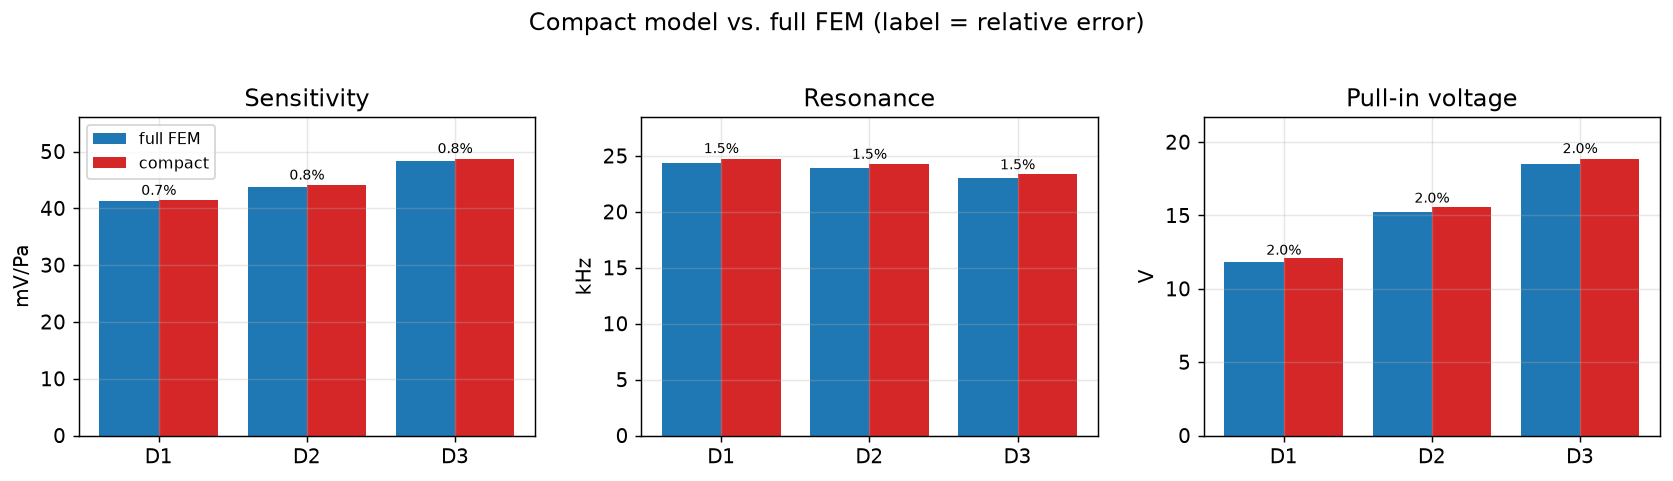
\includegraphics[width=\columnwidth]{fig1_validation.png}
\caption{Compact model vs.\ full FEM across three designs (label = relative
error). Sensitivity, resonance and pull-in agree to $<\!2\%$.}
\label{fig:val}\end{figure}

\begin{figure}[t]\centering
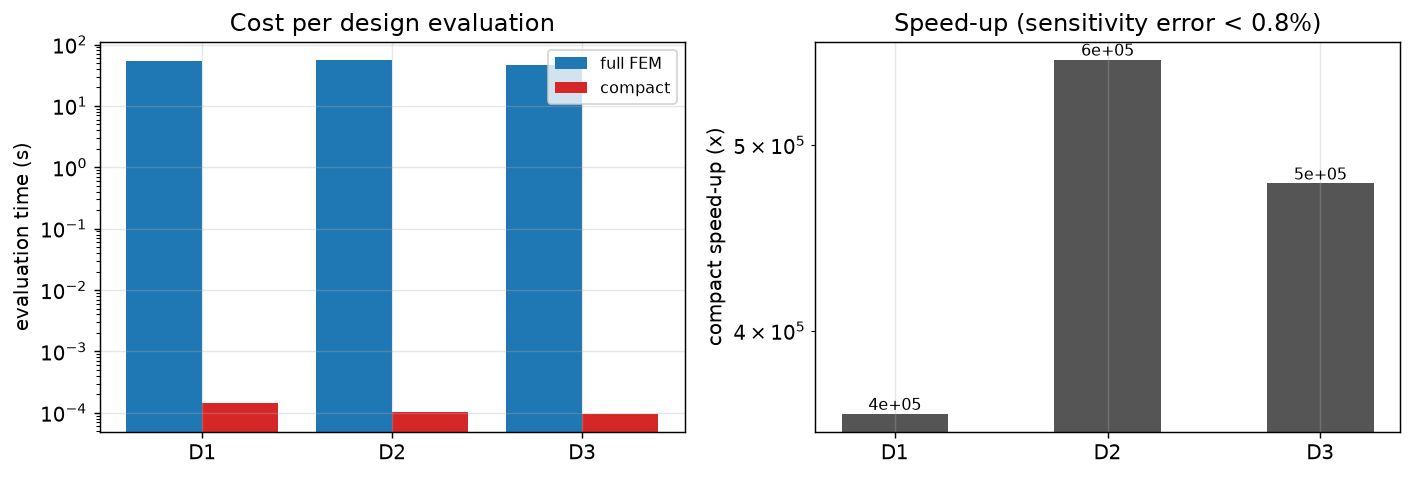
\includegraphics[width=\columnwidth]{fig3_speed_accuracy.png}
\caption{Per-evaluation cost (left) and compact-model speed-up (right); the
closed-form model is $>3\times10^{5}$ faster than FEM at $<\!1\%$ error.}
\label{fig:speed}\end{figure}

\begin{figure}[t]\centering
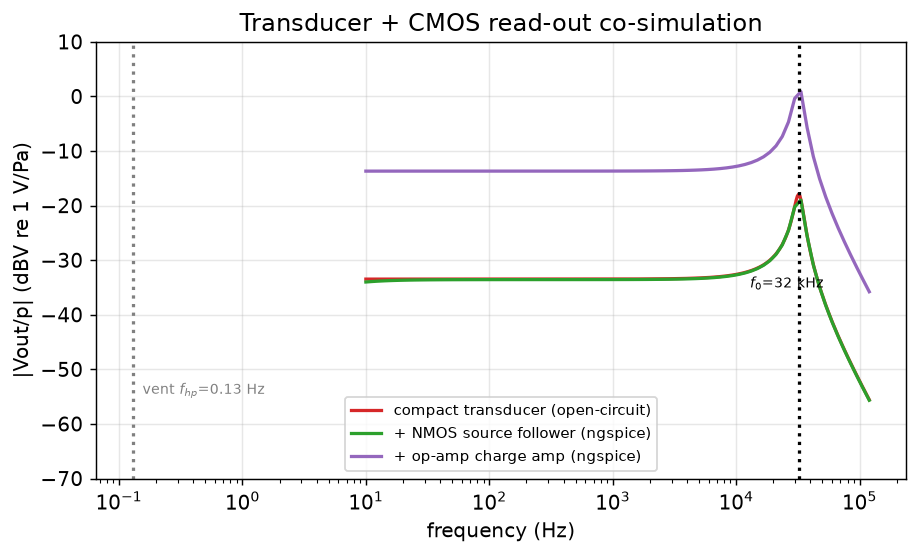
\includegraphics[width=\columnwidth]{fig2_frequency_response.png}
\caption{Transducer + CMOS read-out co-simulation in ngspice. The SPICE
macromodel (red) matches the analytic transducer; the source follower (green)
and charge amplifier (purple) add read-out loading, gain and the electrical
high-pass.}
\label{fig:freq}\end{figure}

\begin{figure}[t]\centering
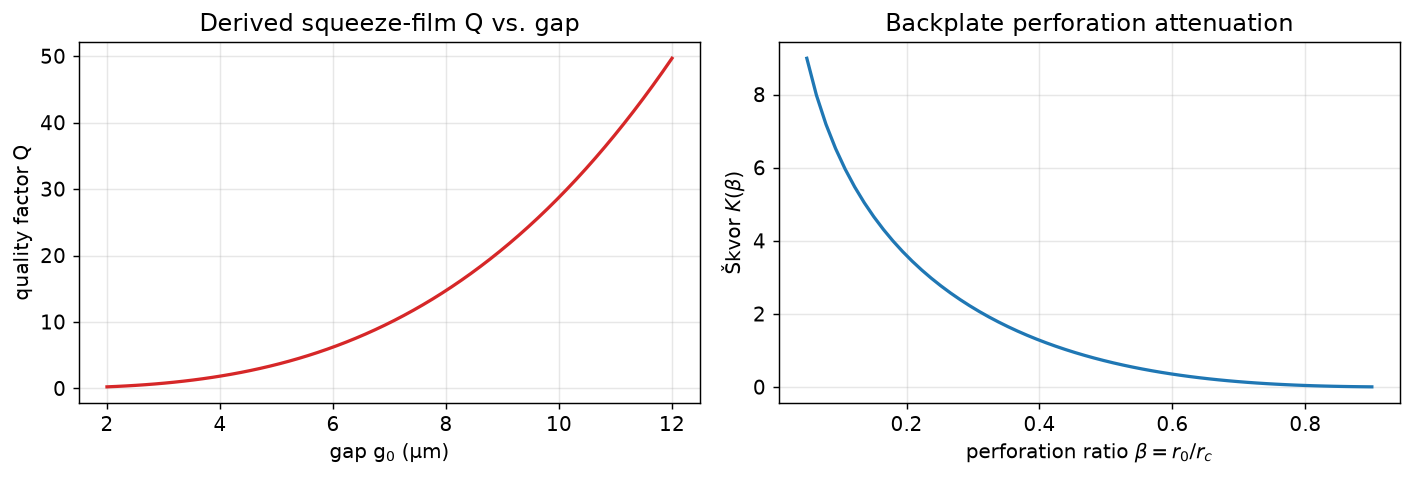
\includegraphics[width=\columnwidth]{fig4_squeeze_film.png}
\caption{Derived squeeze-film quality factor vs.\ gap (left) and the Sk\v{v}or
perforation attenuation $K(\beta)$ (right).}
\label{fig:sqz}\end{figure}

\begin{figure}[t]\centering
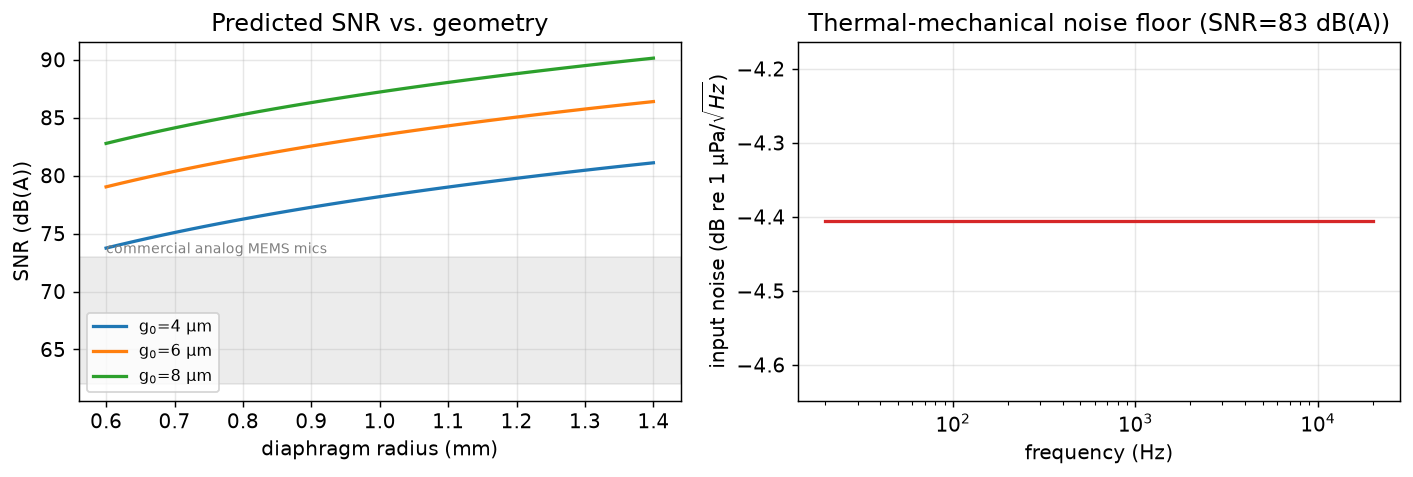
\includegraphics[width=\columnwidth]{fig5_noise_snr.png}
\caption{Predicted A-weighted SNR vs.\ geometry (left) with the commercial band,
and the thermal-mechanical input-noise floor (right).}
\label{fig:noise}\end{figure}

\begin{figure}[t]\centering
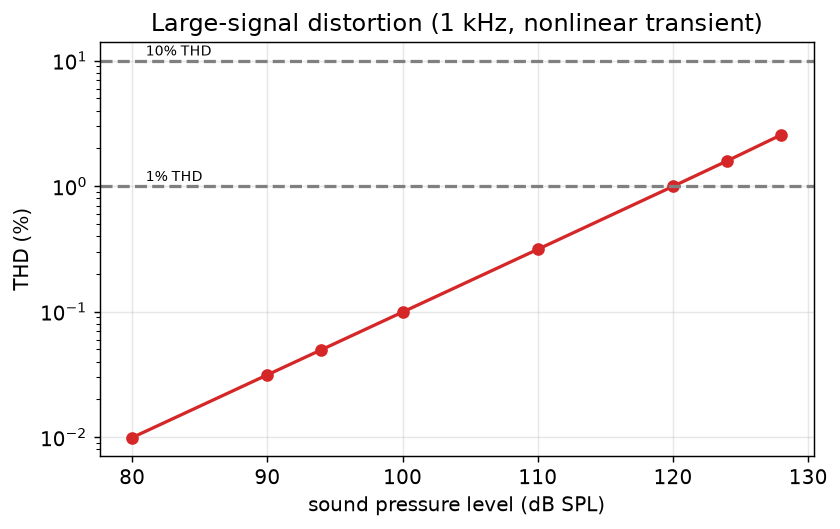
\includegraphics[width=0.86\columnwidth]{fig6_thd.png}
\caption{Large-signal THD vs.\ SPL at $1$~kHz from the nonlinear
constant-charge transient.}
\label{fig:thd}\end{figure}

\begin{figure}[t]\centering
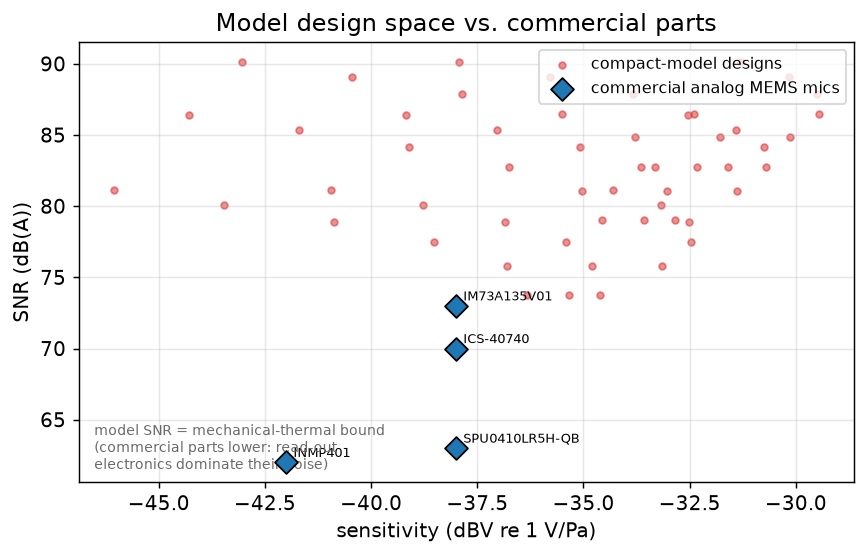
\includegraphics[width=0.9\columnwidth]{fig7_anchors.png}
\caption{Compact-model design space vs.\ published analog MEMS-microphone specs.}
\label{fig:anchor}\end{figure}

\section{Conclusion}
We presented a physically-derived, largely closed-form compact model of a
capacitive MEMS microphone and its Verilog-A/SPICE realization. The circular-mode
capacitance $C(q)=(\varepsilon A/q)\ln[g_0/(g_0-q)]$ makes sensitivity and
pull-in analytic; a Sk\v{v}or squeeze-film term makes the quality factor and the
thermal-mechanical SNR predictive rather than fitted; and a cavity/vent network
sets the audio band. The model tracks a full FE reference to $<\!2\%$ at
$>3\times10^{5}$ speed-up and, unlike FEM, co-simulates with a CMOS front-end,
enabling transducer--circuit co-design. Future work will extend the closed forms
to non-circular and dual-backplate diaphragms, add the squeeze-film gas-spring at
high squeeze number, and calibrate against measured devices.

\begin{thebibliography}{1}
\footnotesize
\bibitem{skvor} R. Sk\v{v}or, ``On the acoustical resistance due to viscous
losses in the air gap of electrostatic transducers,'' \emph{Acustica},
vol.~19, pp.~295--299, 1967.
\bibitem{senturia} S. D. Senturia, \emph{Microsystem Design}. Kluwer, 2001.
\bibitem{starr} J. B. Starr, ``Squeeze-film damping in solid-state
accelerometers,'' in \emph{IEEE Solid-State Sensor and Actuator Workshop},
1990, pp.~44--47.
\bibitem{bay} M. Bao, \emph{Analysis and Design Principles of MEMS Devices}.
Elsevier, 2005.
\bibitem{zuo} C. Zuo \emph{et al.}, ``Lumped-element modeling of capacitive MEMS
microphones,'' \emph{J. Microelectromech. Syst.}, 2019.
\bibitem{verilogams} Accellera, \emph{Verilog-AMS Language Reference Manual},
v2.4.0, 2014.
\bibitem{ngspice} H. Vogt \emph{et al.}, \emph{ngspice, the open-source SPICE
circuit simulator}, \url{https://ngspice.sourceforge.io}.
\end{thebibliography}

\end{document}
